\begin{frame}{A miniHPC - CarpentriesOffline}
	\begin{columns}[T]
		\begin{column}[c]{.6\textwidth}
			\begin{itemize}
				\item Pixie: Raspberry Pi 4s, one login node, five compute nodes, one access point
				\item The same open source software stack as many HPCs: Slurm, lmod, munge
				\item Running Workshops and Hackerthons
					\begin{itemize}
						\item Lesson to build a login node and a compute node
						\item Adapt HPC lesson for Pixie
						\item Networking lesson
					\end{itemize}				
			\end{itemize}
		\end{column}
		
		\begin{column}[c]{.5\textwidth}
			\begin{figure}
				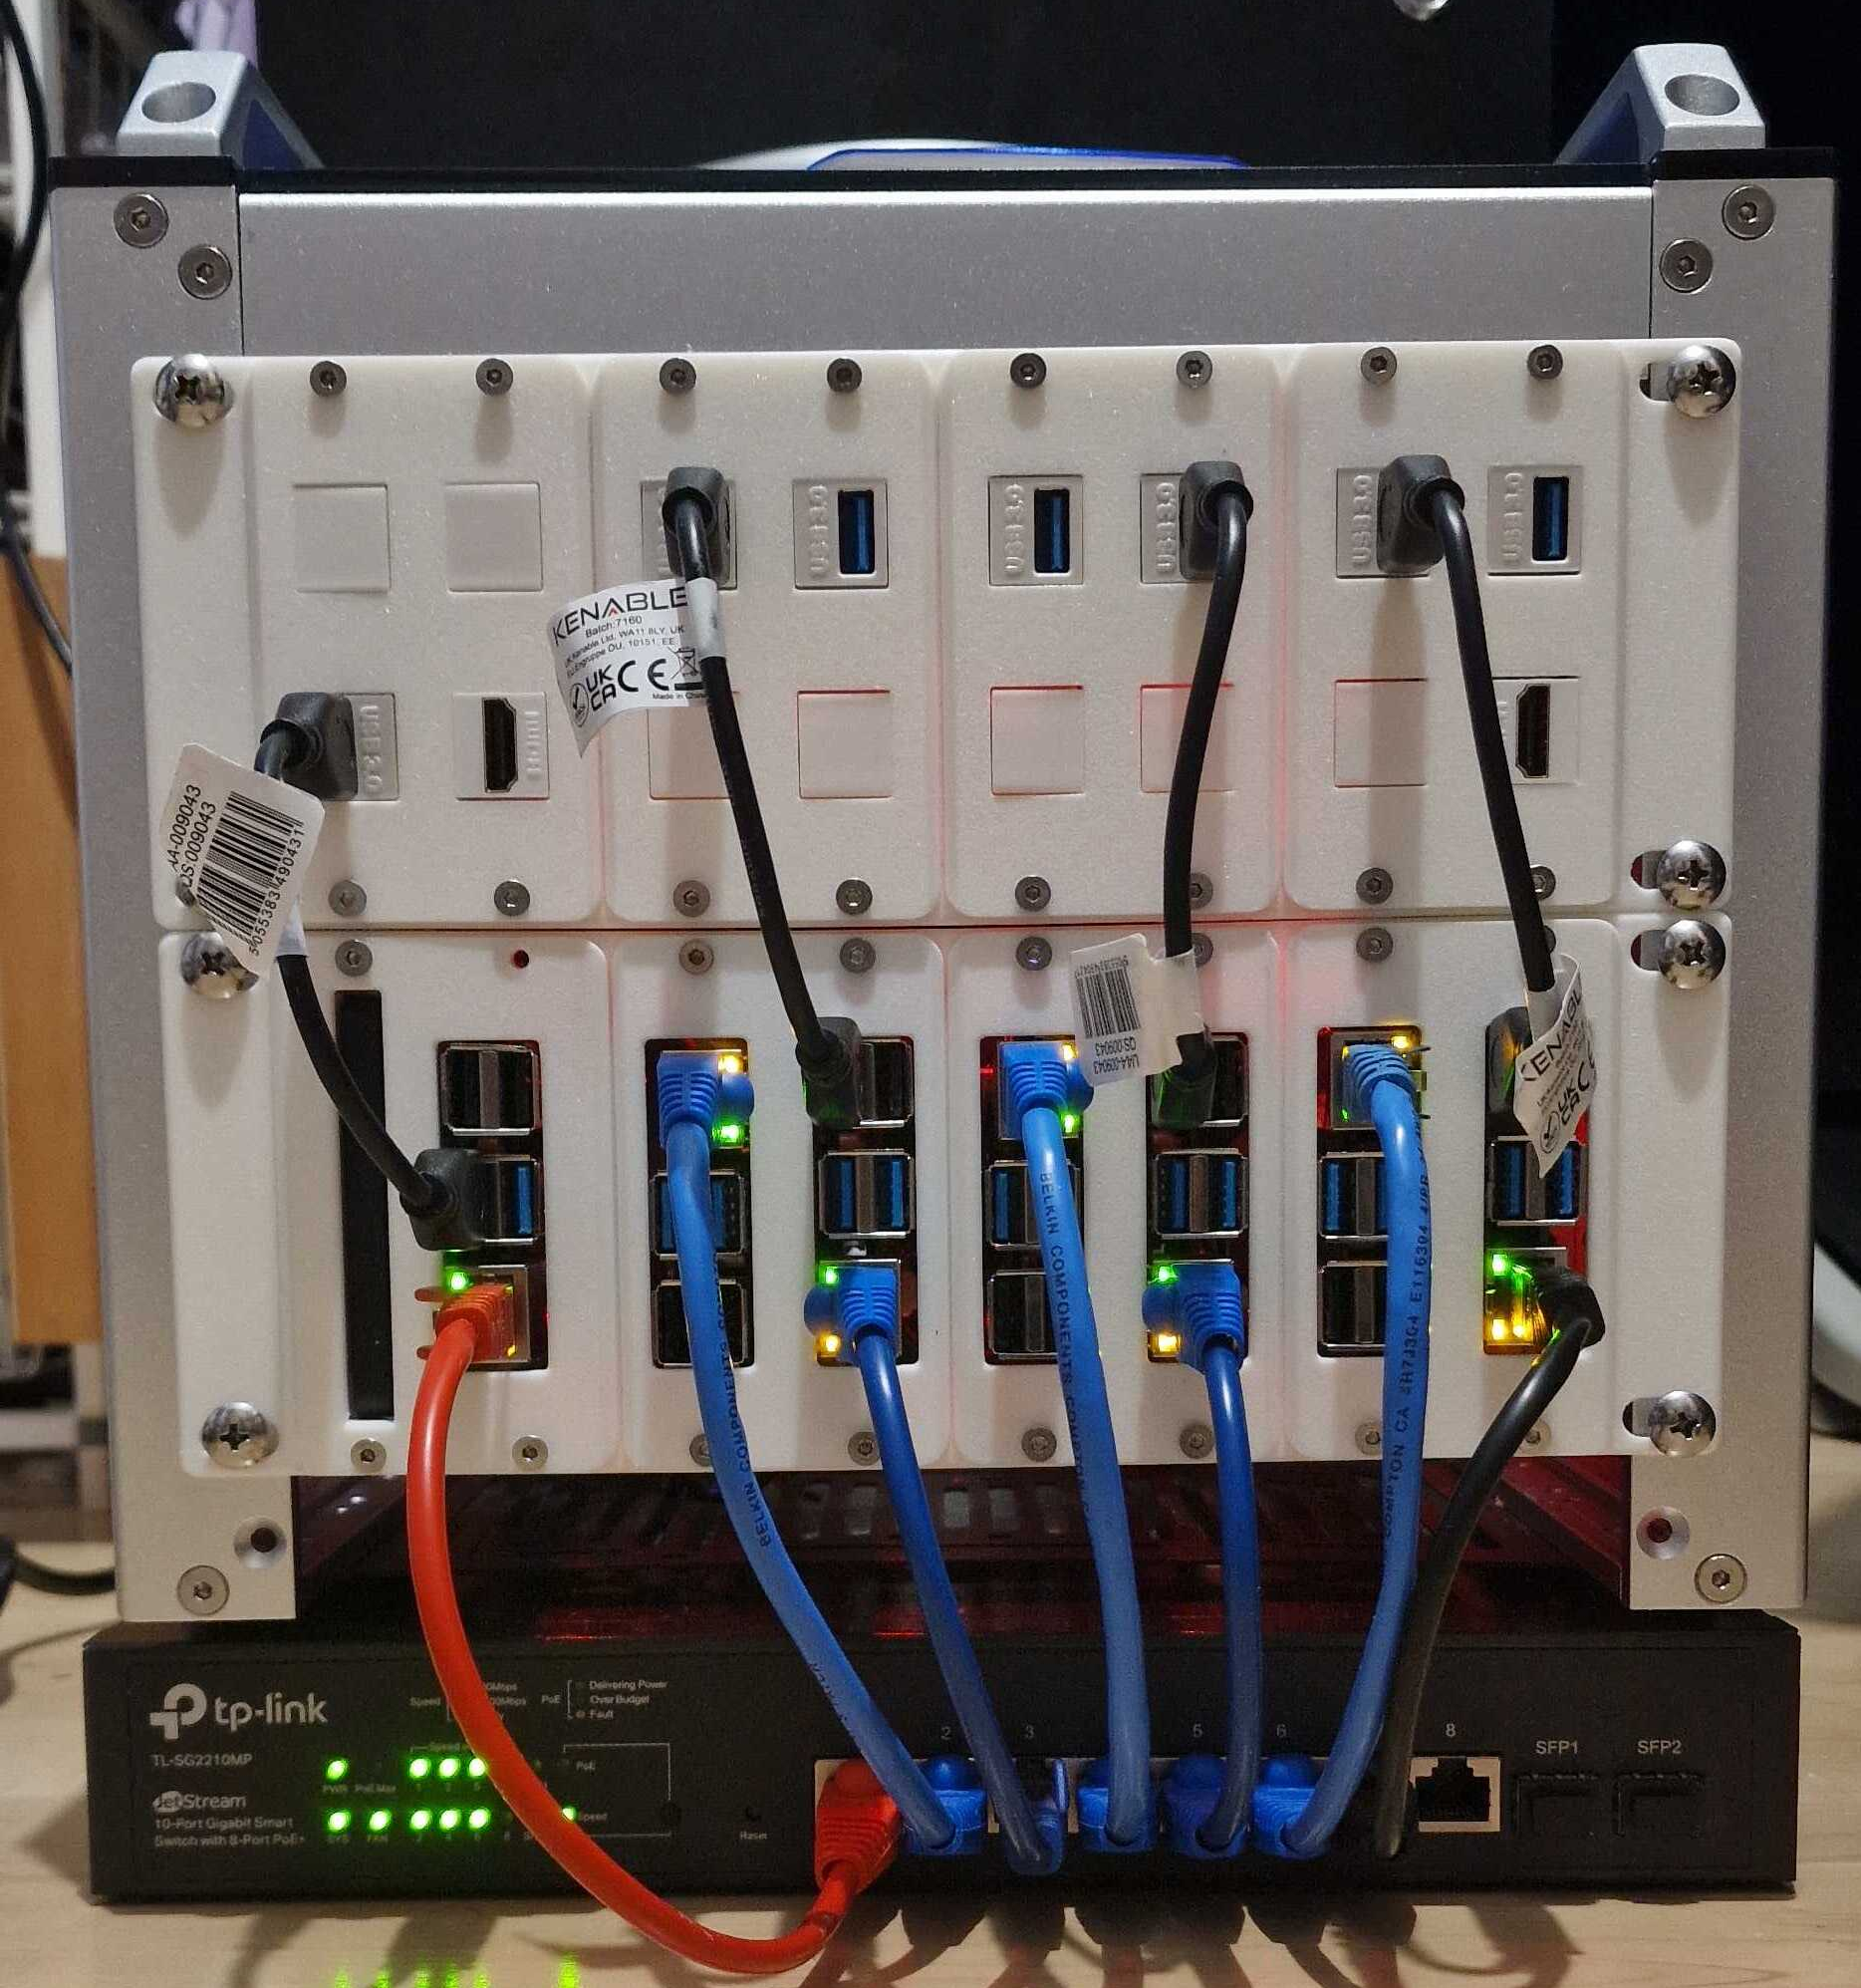
\includegraphics[width=.4\columnwidth]{images/mini-HPC-proto3.png} 
				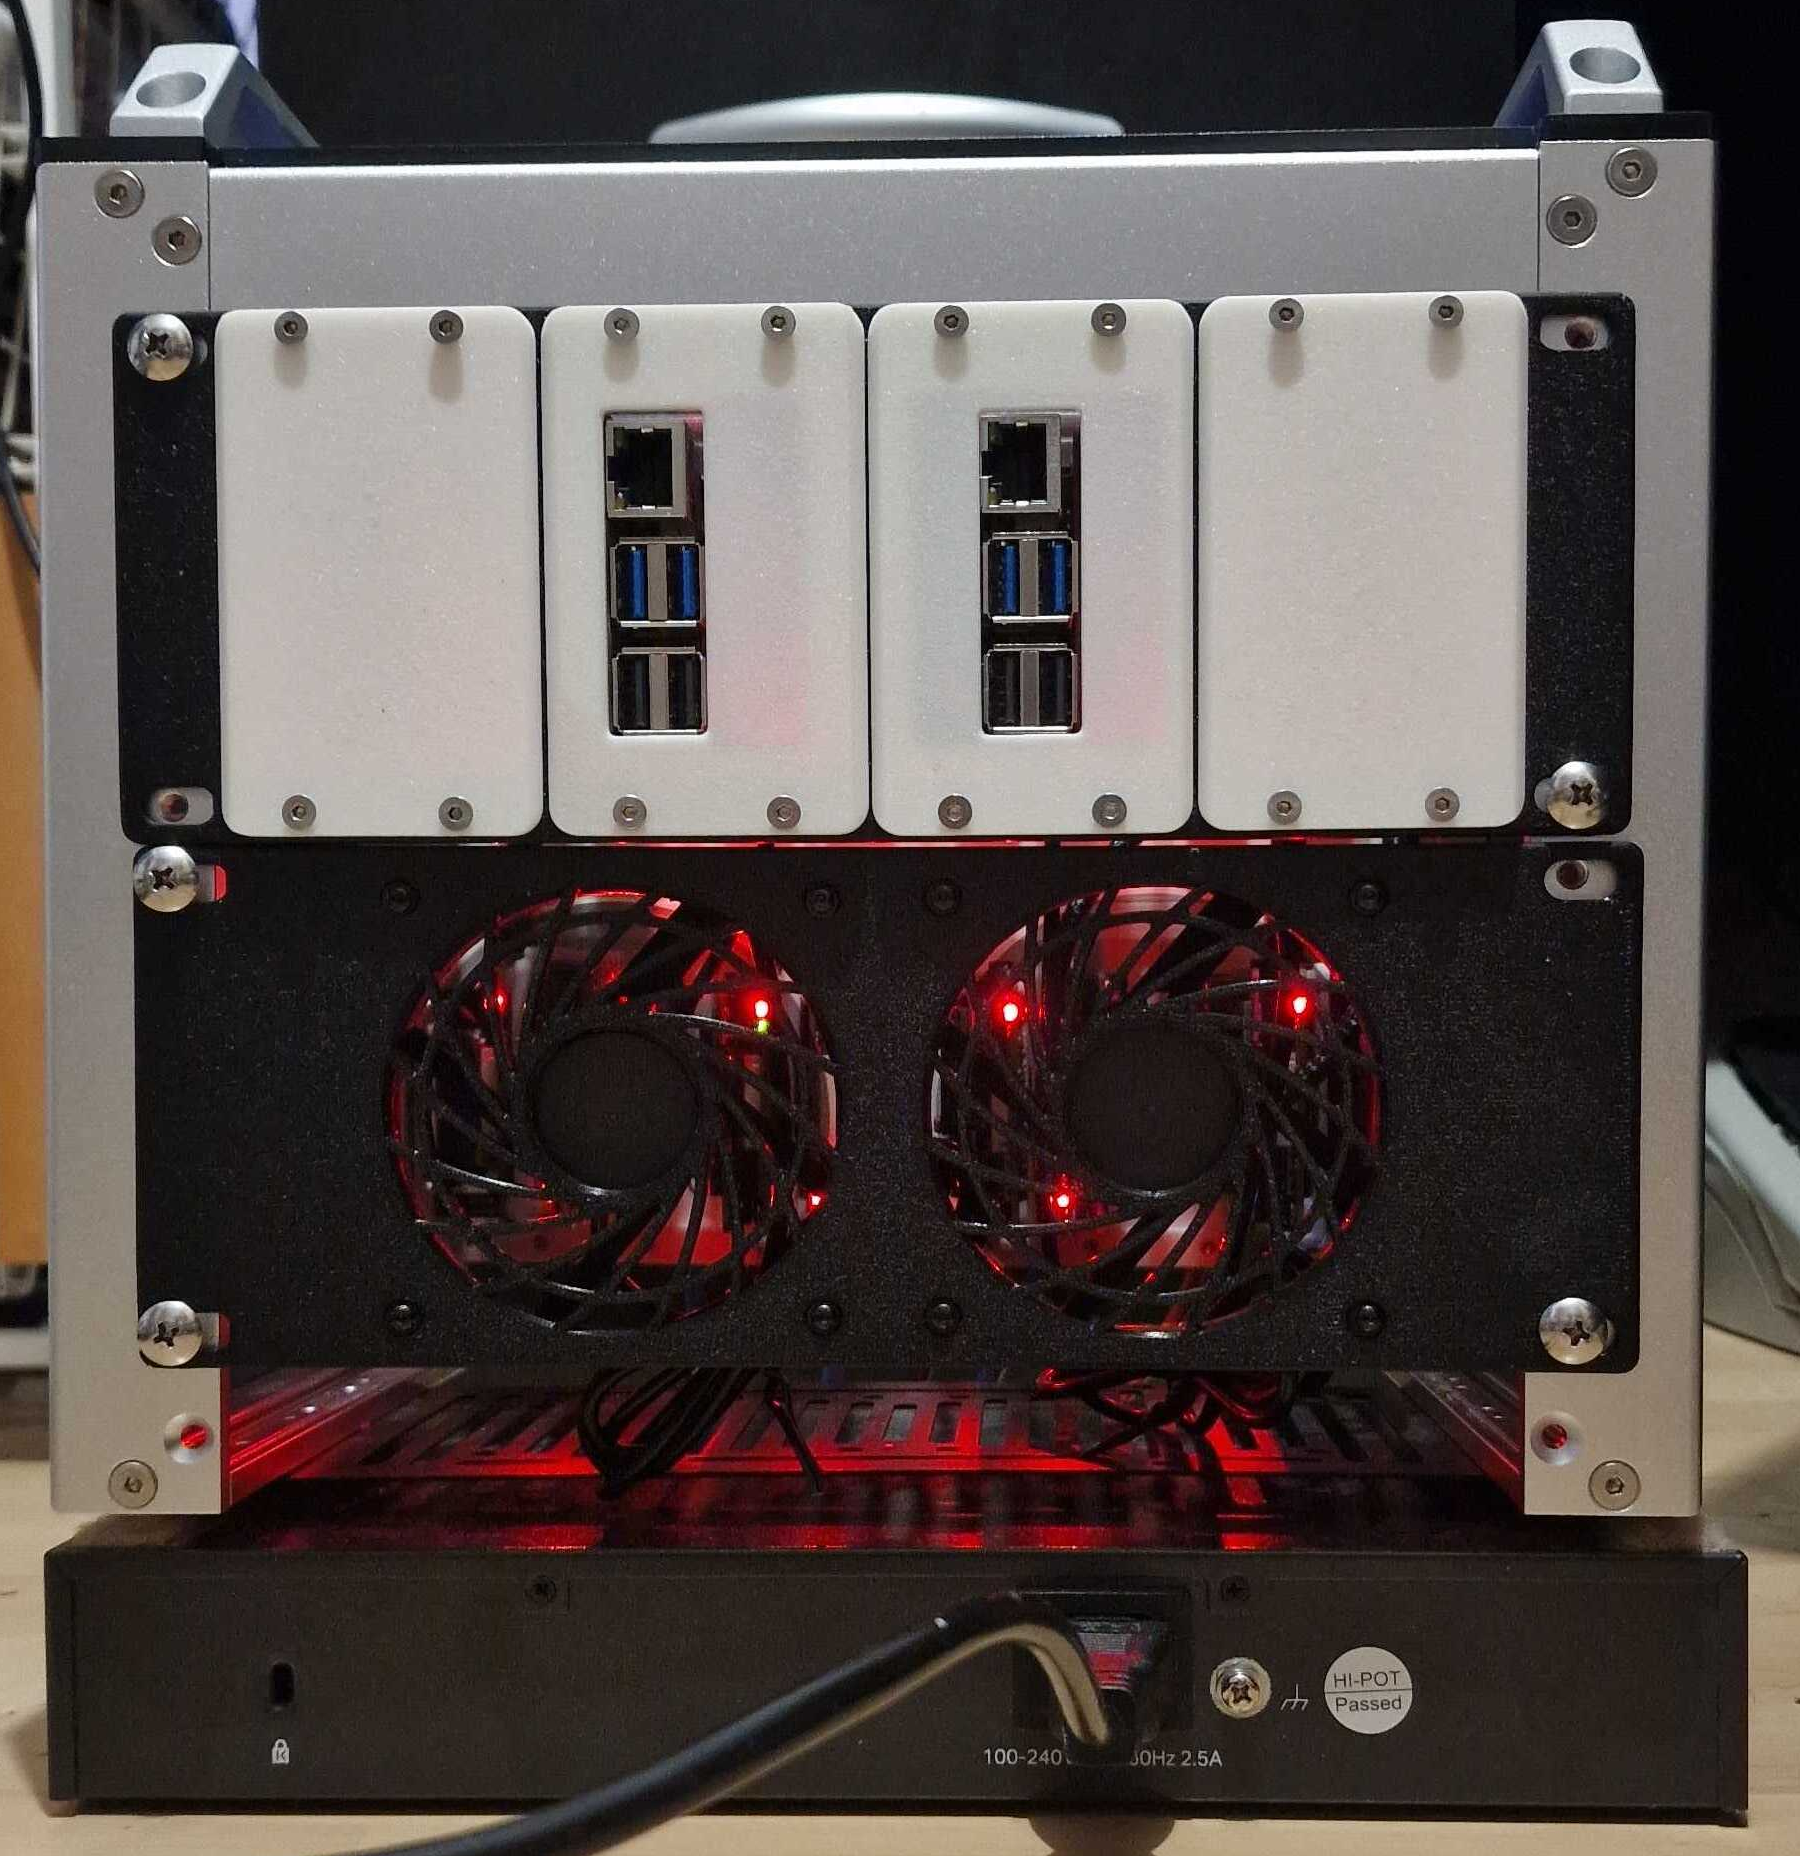
\includegraphics[width=.4\columnwidth]{images/mini-HPC-proto3_back.png}
				\caption*{Front and Back}
			\end{figure}
			\vspace{-2em} 
			\begin{figure}
				
\includegraphics[width=.2\columnwidth]{images/logo.png} 
			\end{figure}
		\end{column}
	\end{columns}
	
\end{frame}